
\documentclass{beamer}
\usepackage{framed}
\usepackage{geometry}
\usepackage{lipsum}  % to generate placeholder text (lines)
\usepackage{graphicx}
\usetheme{metropolis}
\geometry{paperwidth=6.25cm,paperheight=9cm}
\setbeamertemplate{navigation symbols}{}
\setbeamertemplate{frametitle}[default][center]
\setbeamersize{text margin left=5pt,text margin right=5pt}
\usefonttheme{serif}
\setbeamerfont{frametitle}{size=\footnotesize}
\definecolor{codegreen}{rgb}{0,0.6,0}
\definecolor{codered}{rgb}{0.6,0,0}
\setbeamercolor{frametitle}{bg=white,fg=black}
\setbeamertemplate{background}{
    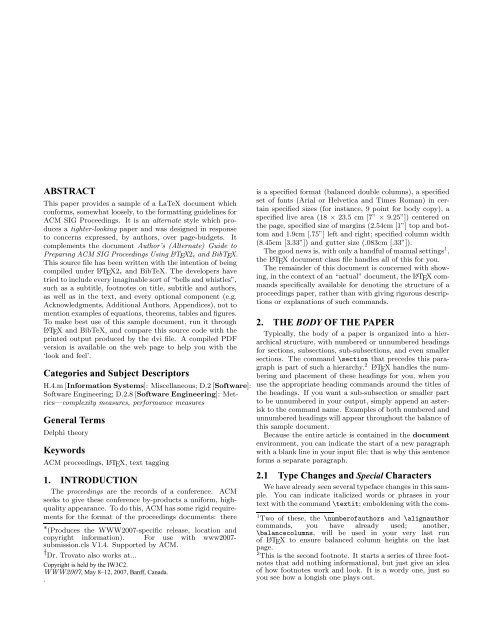
\includegraphics[width=\paperwidth,height=\paperheight]{acm_background.jpg}
}
\addtolength{\headsep}{0.35cm}
\begin{document}
\begin{frame}[plain]
\frametitle{Enhancing Comprehension and Navigation in Jupyter Notebooks with Static Analysis}
\end{frame}
\begin{frame}[plain]
\frametitle{Flowdroid: Precise context, flow, field, object-sensitive and lifecycle-aware taint analysis for android apps}
\end{frame}
\begin{frame}[plain]
\frametitle{A qualitative analysis of android taint-analysis results}
\end{frame}
\begin{frame}[plain]
\frametitle{Enhancing human-in-the-loop adaptive systems through digital twins and VR interfaces}
\end{frame}
\begin{frame}[plain]
\frametitle{A large-scale study of usability criteria addressed by static analysis tools}
\end{frame}
\begin{frame}[plain]
\frametitle{CrySL: An Extensible Approach to Validating the Correct Usage of Cryptographic APIs}
\end{frame}
\begin{frame}[plain]
\frametitle{Boomerang: Demand-driven flow-and context-sensitive pointer analysis for java}
\end{frame}
\begin{frame}[plain]
\frametitle{VREUD-an end-user development tool to simplify the creation of interactive VR scenes}
\end{frame}
\begin{frame}[plain]
\frametitle{Are Neural Bug Detectors Comparable to Software Developers on Variable Misuse Bugs?}
\end{frame}
\begin{frame}[plain]
\frametitle{Automated cell header generator for Jupyter notebooks}
\end{frame}
\begin{frame}[plain]
\frametitle{TaintBench: Automatic real-world malware benchmarking of Android taint analyses}
\end{frame}
\begin{frame}[plain]
\frametitle{Magpiebridge: A general approach to integrating static analyses into ides and editors (tool insights paper)}
\end{frame}
\begin{frame}[plain]
\frametitle{Sootfx: A static code feature extraction tool for java and android}
\end{frame}
\begin{frame}[plain]
\frametitle{Fully-featured anonymous credentials with reputation system}
\end{frame}
\begin{frame}[plain]
\frametitle{Context-, flow-, and field-sensitive data-flow analysis using synchronized pushdown systems}
\end{frame}
\begin{frame}[plain]
\frametitle{Static Analysis for Android GDPR Compliance Assurance}
\end{frame}
\begin{frame}[plain]
\frametitle{Forward-secure 0-RTT goes live: implementation and performance analysis in QUIC}
\end{frame}
\begin{frame}[plain]
\frametitle{Benchmark Fuzzing for Android Taint Analyses}
\end{frame}
\end{document}
